% Poster based on beamerposter.  For more information, see:
% http://www-i6.informatik.rwth-aachen.de/~dreuw/latexbeamerposter.php

\documentclass[final,svgnames,dvipsnames,table]{beamer}
\mode<presentation>{
  \usetheme{HongKong}
}
\usepackage[orientation=portrait,size=a0,scale=1.2]{beamerposter}
%\usepackage[french]{babel}   % "babel.sty" + "french.sty"
\graphicspath{{./}{../figs/}}
\usepackage[utf8]{inputenc}
\usepackage{multicol}
\usepackage{subfigure}
\usepackage{caption}
%\usepackage{subcaption}


%\usepackage{eurosym}
\usepackage{MnSymbol}
\usepackage{tikz}
\usetikzlibrary{arrows,shapes, calc}
\usepackage{xcolor}
\usepackage{array}
\usepackage{hyperref}
\usepackage{cleveref}
%% \usepackage[natbib=true, bibstyle=authoryear, maxnames=2,
%%   citestyle=authoryear-comp]{biblatex}
%% \bibliography{huynh.2016.icpr}
\usepackage{amsmath,,amssymb,amsfonts}
\usepackage{stmaryrd}
\usepackage{tabularx}

\usepackage{relsize}
\usepackage{setspace}

\usepackage{pifont}% http://ctan.org/pkg/pifont
\newcommand{\cmark}{\ding{51}}%
\newcommand{\xmark}{\ding{55}}%

\usepackage{multirow, multicol}
%\usepackage[usenames,dvipsnames,svgnames,table]{xcolor}


%\newcommand{\etal}{{\it et al.}\xspace}

%\usepackage[numbers,sectionbib]{natbib}

% Specific definitions
\definecolor{bglayer}{named}{ta3aluminium}

%\setbeamercolor{block body}{fg=red}
%\setbeamercolor{block itemize item example}{fg=red}
%\setbeamercolor*{block title example}{fg=red}
%\AtBeginEnvironment{exampleblock}{\setbeamercolor{itemize item subitem}{fg=red}}
%\setbeamercolor{local structure itemize item}{fg=red}

\usepackage{xspace}

\newcommand{\Lab}{{\ensuremath{L a^{*} b^{*}}}\xspace}


\title{%\fontsize{64}{60}\selectfont
  \vskip36pt Spherical fluorescent particle segmentation and tracking in 3D confocal microscopy \\[16pt]
  %\texorpdfstring{\colorbox{yellow}{\color{red}{~A Mathematical Morphology Approach~}}}{ } 
  }
\author{\'{E}lodie Puybareau\inst{1,2} \and Edwin Carlinet\inst{1} \and Alessandro Benfenati\inst{2} \and Hugues Talbot\inst{2,3} \\}

\institute{
EPITA Research and Development,
14-16 rue Voltaire, F-94276 Le Kremlin-Bicetre
\and
Université Paris-Est, ESIEE Paris, 2 boulevard Blaise-Pascal, F-93162 Noisy-le-Grand
\and
CentraleSupelec, Centre de Vision Numérique, INRIA équipe OPIS, 3 rue Joliot-Curie, F-91190
Gif-sur-Yvette.\\
}

\date{ISMM 2019 --- Athens, Greece --- October 7-10, 2018}

\logoleft{%
  \vspace{0.5cm}
  \hspace*{-2.5cm}
\includegraphics[width=10cm]{lrde.png}\\[25pt]
  \vspace*{-3em}
}

\logoright{%
  \vspace*{1.5cm}
  %
\includegraphics[width=10cm]{epita-logo} \\[-35pt]
  \vspace*{-3em}
}
\setbeamertemplate{footline}[text line]{\hfill{}\tiny ICIP 2018 --- Athens, Greece --- October 7-10, 2018}

%\setbeamertemplate{background canvas}{%
%\tikz[remember picture,overlay]{\fill[color=blue] (-70, -70) ++(-1,0.5) rectangle ++(23.5,-26.5);
%  \fill[color=blue] (10, 70) ++(22.5, 0.5) rectangle ++(58,-70);}
%}

\definecolor{MyGray}{rgb}{0.1,0.3,0.4}



\begin{document}
\setbeamertemplate{caption}{\raggedright\insertcaption\par}
%% \usebackgroundtemplate{%
%%   \tikz[remember picture, overlay]{
%%     \coordinate [right=1] (midpoint) at (current page.west);
%%     %\filldraw[color=bglayer] (midpoint) ++(0.5, 14) rectangle ++(83,-21);
%%     %\filldraw[color=bglayer] (midpoint) ++(0.5, -27) rectangle ++(83,-22);
%%     %\filldraw[color=bglayer] (midpoint) ++(30, -27) rectangle
%%     %++(53.5,20);
%%     \filldraw[color=bglayer] (midpoint) ++(0.5, -69) rectangle ++(83,83);
%%     \fill[color=white] (current page.south west) rectangle ++(34.5,52);
%%   }
%% }



\begin{frame}[fragile]

\vskip-1em
   \begin{exampleblock}{\bf At a glance}
    \centering

    \vskip .5em
    \begin{figure}
\centering
\subfigure[]{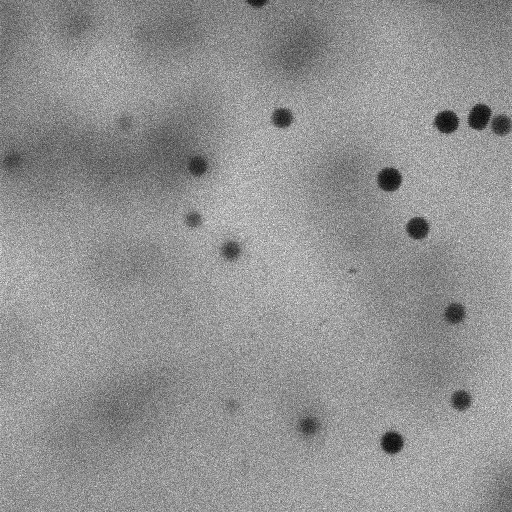
\includegraphics[width =  0.15\linewidth]{images/exp1_t01z5.png}}
\subfigure[]{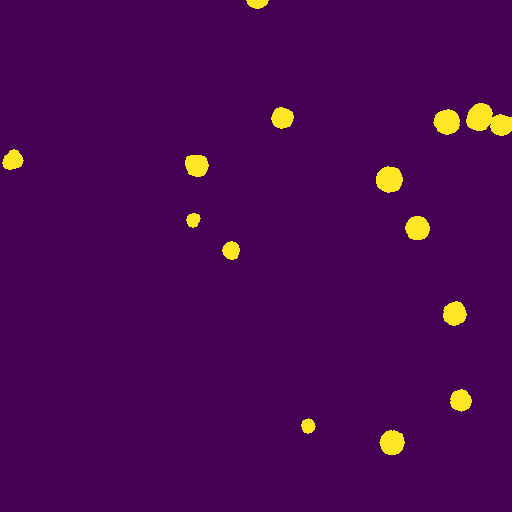
\includegraphics[width =  0.15\linewidth]{images/orig_1.png}}
\subfigure[]{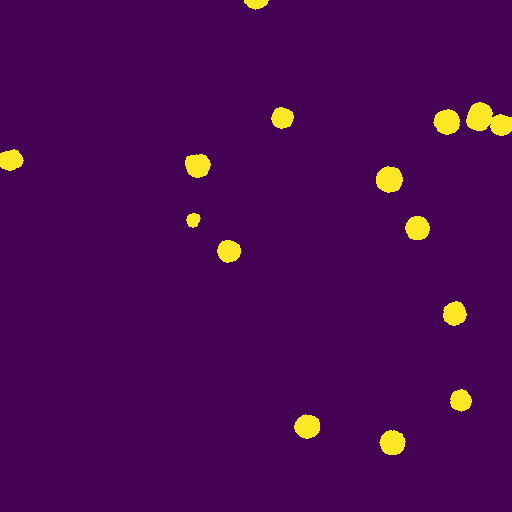
\includegraphics[width =  0.15\linewidth]{images/orig_fermee_1.png}}
%\vspace{0.3em}
\subfigure[]{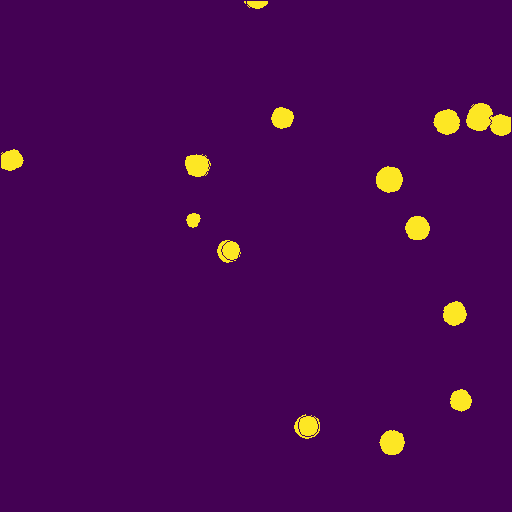
\includegraphics[width =  0.15\linewidth]{images/orig_separ_1.png}}
\subfigure[]{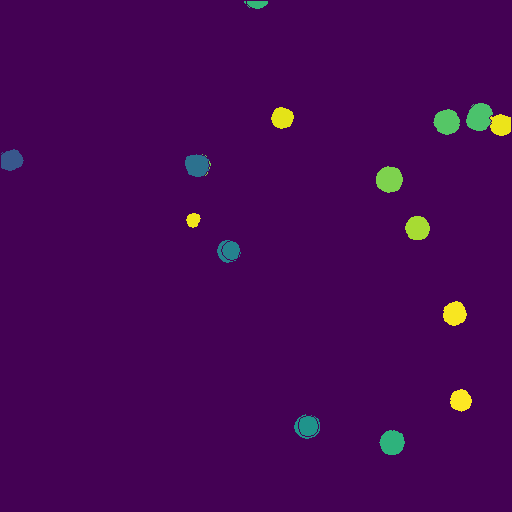
\includegraphics[width =  0.15\linewidth]{images/toto.png}}
\caption{Results of the successive steps: (a) initial image, (b) inital segmentation, (c) 3d regularization, (d) bead separation, (e) individualization and labeling.}
\label{fig:temporal}
\end{figure}
    \begin{multicols}{2}
    \begin{description}
    \item[{\bf ~~Problem:}] ~ %
      \begin{itemize}
      \item Spherical fluorescent beads are used in many areas of
        physics and biology for positioning and tracking;
      \item not many 3D segmentation methods exist for tracking in
        fluid: the particles move during acquisition due to Brownian
        motion;
      \item radius distribution is known but not precise radius.
      \end{itemize} \bigskip %
      %
    \item[{\bf ~~Why our approach is interesting:}] ~ %
      \begin{itemize}
      \item based on classical mathematical morphology operators~{\color{cyan}\cite{morpho}};
      \item aggregates information from 2D slices to find most likely
        position and radius;
      \item 
      \end{itemize} \bigskip %
      %
    \item[{\bf ~~Conclusion:} ] ~\newline %
      our method is
      \begin{itemize}
      \item 
      \item 
      \item 
      \end{itemize}
    \end{description}
    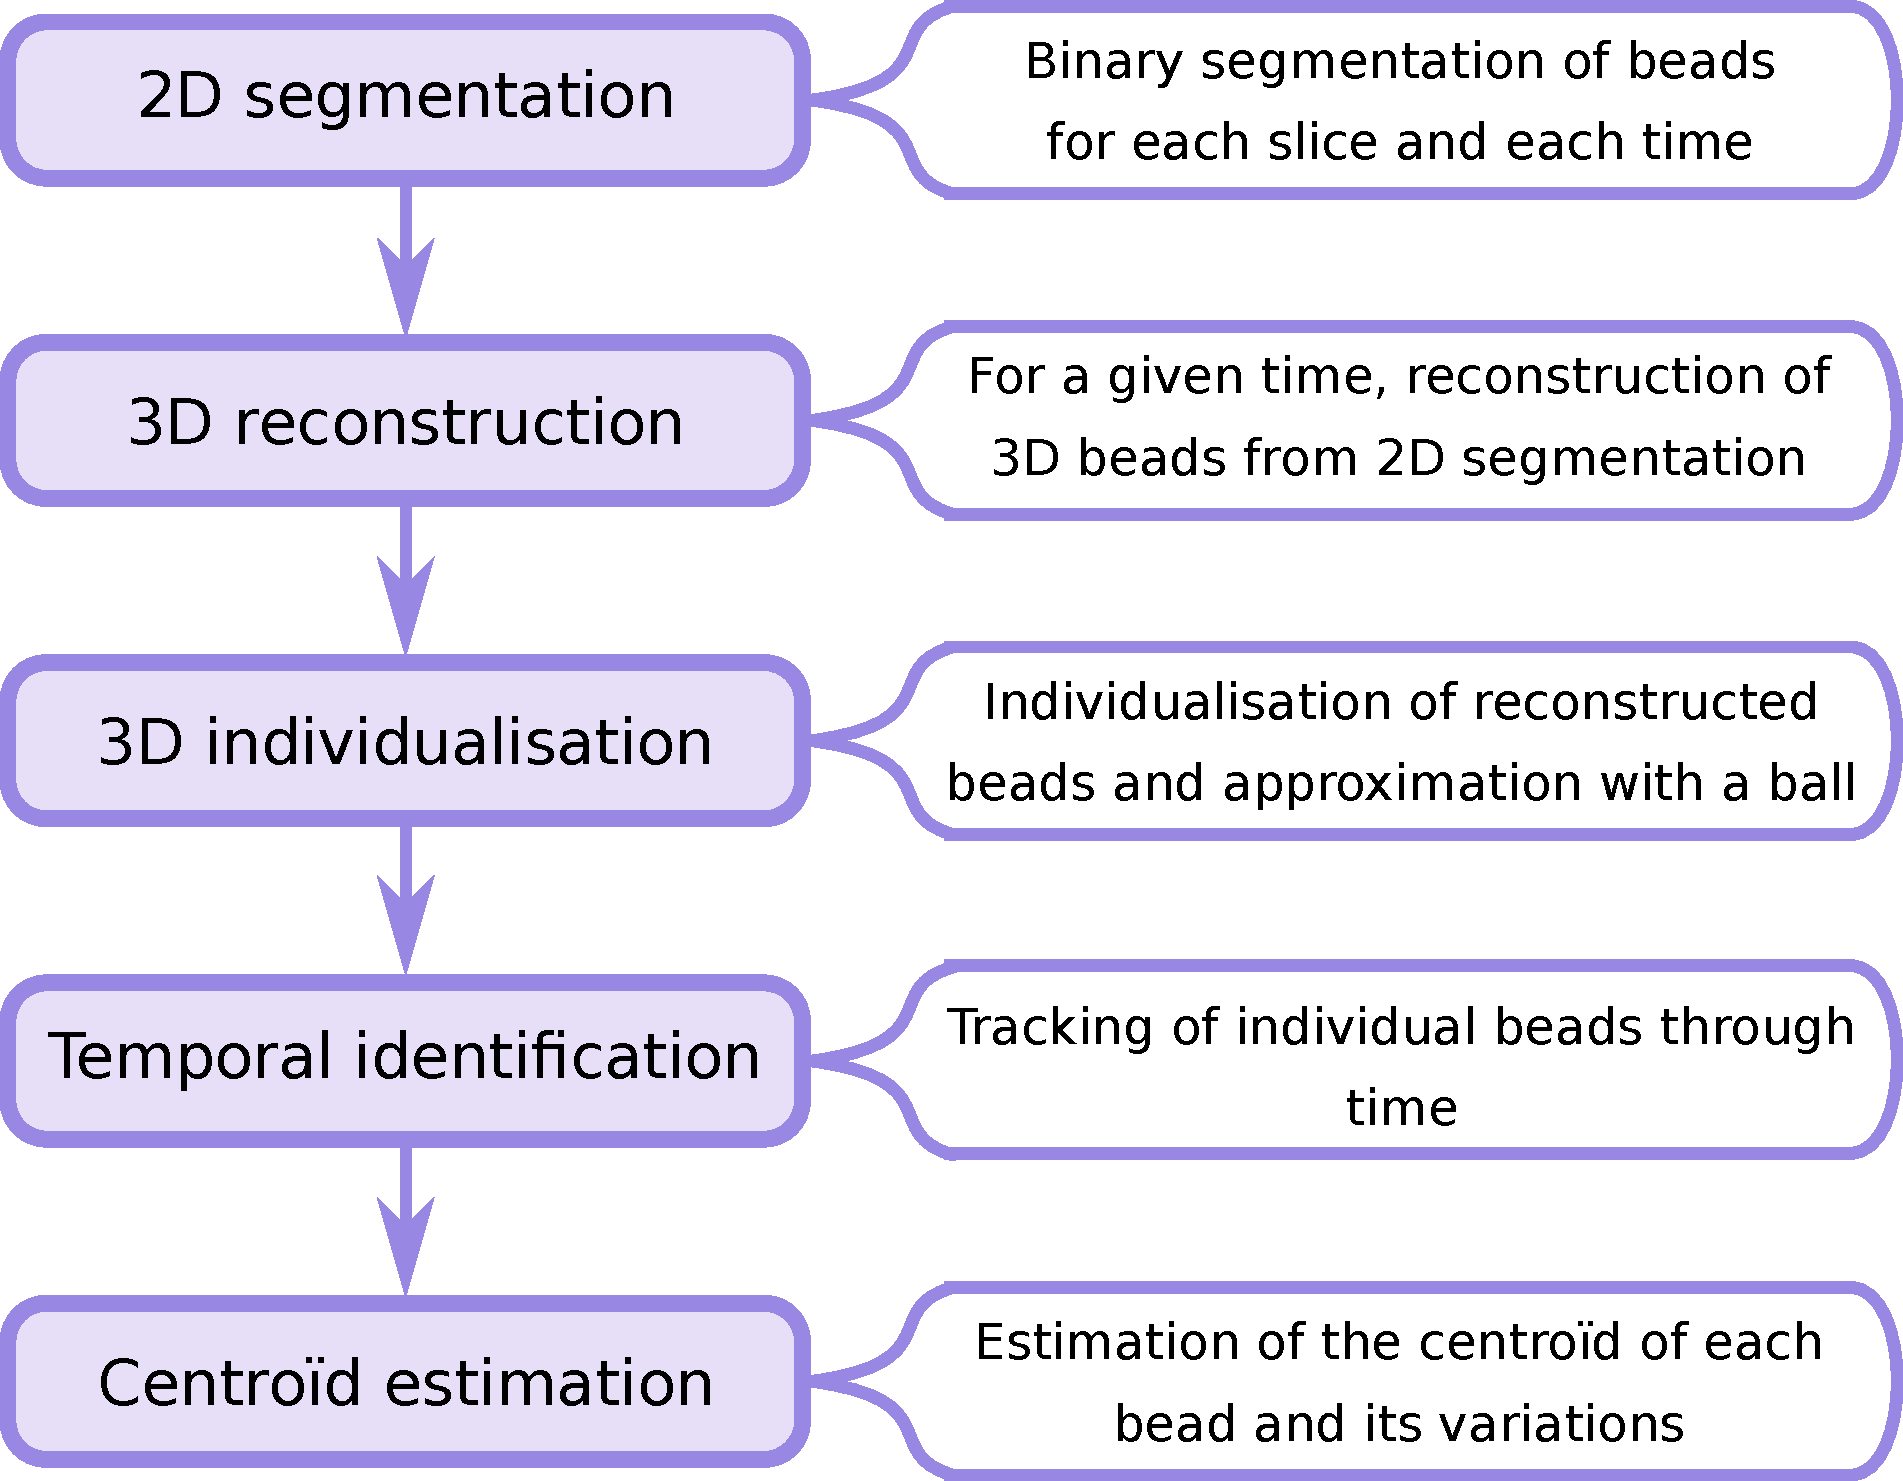
\includegraphics[width = 0.6\linewidth]{images/flowchart.pdf}
    \end{multicols}
   \end{exampleblock}
   
   
  \begin{columns}[t,totalwidth=\textwidth]
    %
    % LEFT
    %
    %\begin{column}{\textwidth}

   %\end{column}
   \begin{column}{0.32\textwidth}
   % ###############################################
   %\vskip .5em
    % ###############################################
    
    \begin{block}{\bf Particle tracking}
      \centering

      \vskip .5em
      \begin{itemize}
          \item 2D Segmentation pipeline: \\ \begin{enumerate}
\item Supression of small local minimas (closing by reconstruction with an initial dilation by a disk of radius 4).
\item Calculation of the min-tree of the previous result.
\item Filtering of nodes by combined criteria (size, grey-level intensity, contrast of component). 
\item Regularisation of the selected blobs.
\end{enumerate}
\begin{figure}
\centering
\subfigure[]{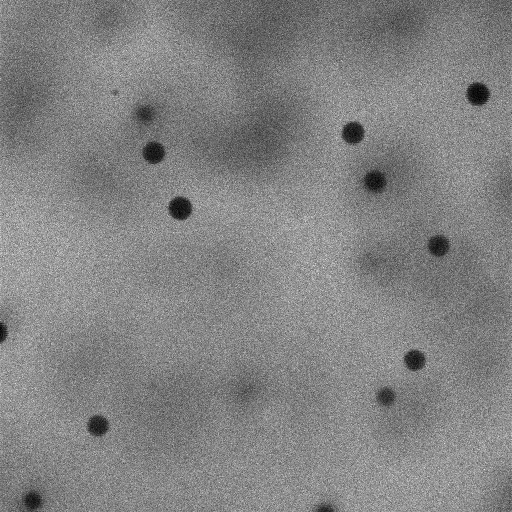
\includegraphics[width =  0.3\linewidth]{images/exp1_t41z4.png}}
\subfigure[]{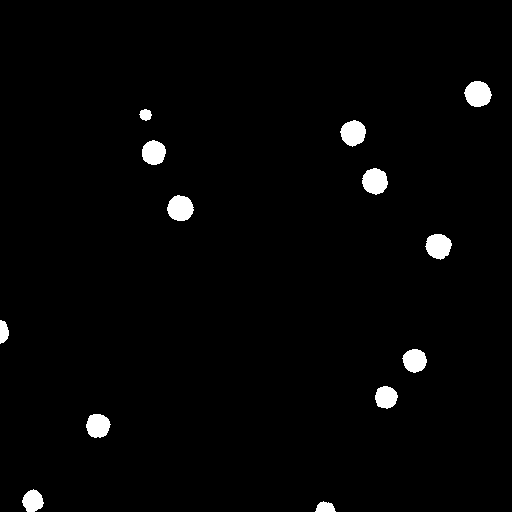
\includegraphics[width =  0.3\linewidth]{images/exp1_t41z4_bin.png}}
\subfigure[]{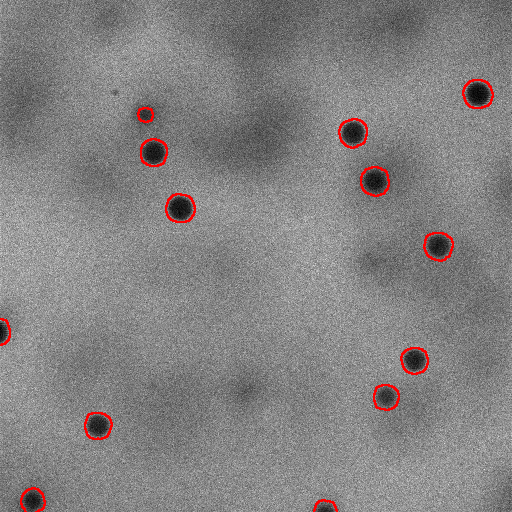
\includegraphics[width =  0.3\linewidth]{images/surimp_exp1_t41z4.png}}
\caption{Illustration of the segmentation procedure: (a) initial image, (b) result of the segmentation described in the text,  (c) overlay of the segmentation on the initial image.}
\label{fig:seg1}
\end{figure}
        \item 3D regularization: 2D closing with a disk of radius 1 in the $xz$ planes.
        \item 3D individualization: beads markers are extracted using the distance transform and a watershed is applied and result is filtered using a volume criterion.
        \item Temporal identification: labels are propagated between two consecutive frames $t$ and $t-1$ by finding the intersection between the beads at $t$ and $t-1$ used for the reconstruction by dilation. The remaining unlabeled beads are given new labels.
      \end{itemize}
     

%      \begin{tabular}{c@{\hskip 1em}c@{\hskip 1em}c@{\hskip 1em}c}
%        \rotatebox{90}{~~~~~~~~~~~Input} &
%        \includegraphics[trim=120 708 500 120, clip, width=.23\linewidth]{defocus2} &
%       \includegraphics[trim=120 708 500 120, clip, width=.23\linewidth]{brighter} &
%        \includegraphics[trim=120 708 500 120, clip, width=.23\linewidth]{IMG_0336_dark}\\
%        %
%        \rotatebox{90}{~~~~~~~~~Chunks} &
%        \includegraphics[width=.23\linewidth]{defocus2_chunks} &
%        \includegraphics[width=.23\linewidth]{brighter_chunks} &
%         \includegraphics[width=.23\linewidth]{IMG_0336_dark_wst}\\
%         %
%        \rotatebox{90}{~~~~~~Final decision} &
%         \includegraphics[width=.23\linewidth]{defocus2_out} &
%         \includegraphics[width=.23\linewidth]{brighter_out} &
%         \includegraphics[width=.23\linewidth]{IMG_0336_dark_out}\\
%         %
%         &
%         Defocus + flare & Noise & Low-light env \\
%      \end{tabular}
    \end{block}
    \end{column}
    %
    %\hfill
    %
    % RIGHT
    %
    \begin{column}{0.32\textwidth}
%      \begin{block}{\bf Step by step}
%
%        \vskip .5em
%
%        ~~~
%        \begin{minipage}{.154\textwidth}\centering
%          \includegraphics[width=.9\textwidth]{IMG_0336}
%          
%          Input
%        \end{minipage}
%        \hfill
%        \begin{minipage}{.154\textwidth}\centering
%          \includegraphics[width=.9\textwidth]{IMG_0336_temp_lab_filtered}
%
%          $La^{*}b^{*}$ filtered
%        \end{minipage}
%        \hfill
%        \begin{minipage}{.154\textwidth}\centering
%          \includegraphics[width=.9\textwidth]{IMG_0336_temp_grad}
%          
%          Gradient
%        \end{minipage}
%        \hfill
%        \begin{minipage}{.154\textwidth}\centering
%          \includegraphics[width=.9\textwidth]{IMG_0336_temp_wst_basins}
%          
%          Basins
%        \end{minipage}
%        \hfill
%        \begin{minipage}{.154\textwidth}\centering
%          \includegraphics[width=.9\textwidth]{IMG_0336_temp_chunks_selection_alt}
%
%          Chunks
%        \end{minipage}
%        \hfill
%        \begin{minipage}{.154\textwidth}\centering
%          \includegraphics[width=.9\textwidth]{IMG_0336_out}
%          
%          Decision
%        \end{minipage}
%        ~~~
%     \end{block}


   % ###############################################
   %\vskip .5em
    % ###############################################
    
      \begin{minipage}{1\textwidth}\centering
        \begin{block}{\bf Position estimation}
%      \begin{description}
        \begin{itemize}
        \item Centroid estimation in 2D 
        \item Centroid estimation in 3D with known bead radius
        \item Centroid estimation in 3D with imprecise bead radius
      \end{itemize}
%        \end{description}
        \end{block}
        \end{minipage}

        %\vskip .2em
        
        % ######################################################
            \end{column}
    %
    %\hfill
    %
    % RIGHT
    %
    \begin{column}{0.32\textwidth}
        \begin{block}{\bf \color{white} Results on simulations}
          \null\centering\relax

          \newcommand{\bl}{\color{black}}
          
        \vskip -1em

\resizebox{.67\linewidth}{!}{
\begin{tabular}{|c|cccc|c|}
    \hline 
    \bl {\bf Method} & \bl {\bf ~set\#1~} & \bl {\bf ~set\#2~} & \bl {\bf ~set\#3~} & \bl {\bf ~set\#4~} & \bl {\bf ~runtime~~}\\
    \hline\hline
       \bl  {Xu et al.}~{\color{cyan}\cite{xu}} & \bl 0.997 & \bl 0.987 & \bl 0.999 & \bl 0.994 & \bl \textgreater 1min\\ % global score = .9816
    \bl {LRDE \@ SmartDoc} & \bl 0.987 & \bl 0.977 & \bl 0.989 & \bl 0.984 & \bl \textgreater 1min\\
%    {ISPL-CVML} & \bl 0.987 & \bl 0.965 & \bl 0.985 & \bl 0.977 \\
    \bl {Leal et al.~{\color{cyan}\cite{leal}} (best)} & \bl 0.961 & \bl 0.944 & \bl 0.965 & \bl 0.930 & \bl 0.43s \\
    \bl {\it SmartDoc average}~{\color{cyan}\cite{burie}} & \bl \it 0.946 & \bl \it 0.903 & \bl \it 0.938 & \bl \it 0.812 & \bl \it ? \\
    \bl {~~Leal et al.~{\color{cyan}\cite{leal}} (fastest)~~} & \bl 0.921 & \bl 0.849 & \bl 0.909 & \bl 0.840 & \bl 0.10s \\
    \hline
    \bl  {Our} & \bl 0.905 & \bl 0.936 & \bl 0.859 & \bl 0.903 & \bl {\bf 0.04s} \\
    \hline
\end{tabular}
}
        \end{block}
      %\end{minipage}
      %
      \hfill
      %
            \begin{block}{\bf \color{white} Results on real data}
          \null\centering\relax
        %\newcommand{\greencheck{{\color{green}\checkmark}}}

       
          %\newcommand{\bl}{\color{black}}
        \vskip -1em
        \centering
        \begin{itemize}
            \item[\cmark] Correct beads segmentation 
            \item[\cmark] Correct beads identification
            \item[\xmark] Overestimation of beads presence in z-axis;
            \item[\xmark] No ground truth for the diffusion coefficient.
        \end{itemize}
\begin{figure}
\centering
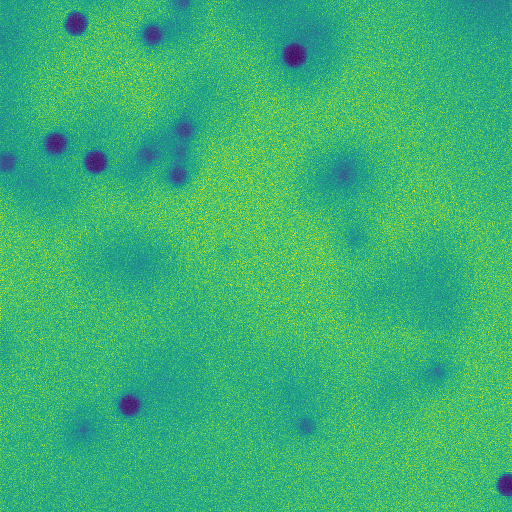
\includegraphics[width = 0.3\linewidth]{images/orig_tot.png}\hspace{0.2em}
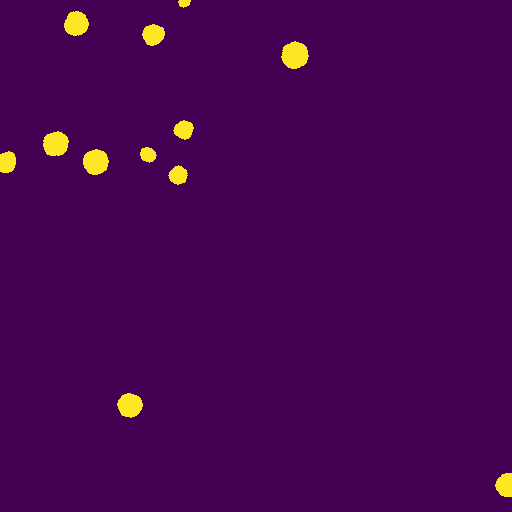
\includegraphics[width = 0.3\linewidth]{images/seg_base_tot.png}\hspace{0.2em}
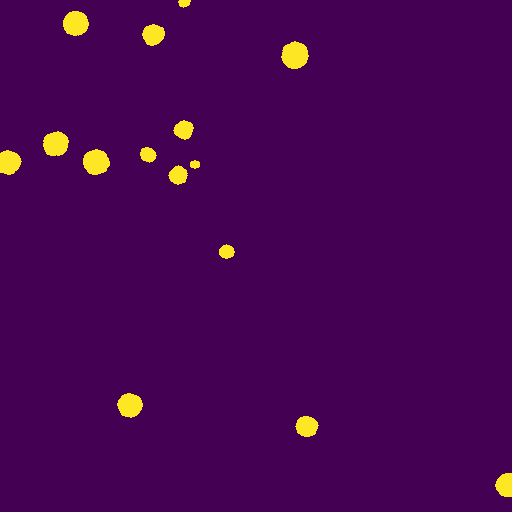
\includegraphics[width = 0.3\linewidth]{images/modif_tot.png}\\
\vspace{0.3em}
\subfigure[]{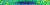
\includegraphics[width = 0.3\linewidth]{images/orig.png}}\hspace{0.2em}
\subfigure[]{
\includegraphics[width = 0.3\linewidth]{images/seg_base.png}}\hspace{0.2em}
\subfigure[]{
\includegraphics[width = 0.3\linewidth]{images/modif.png}}\\
\caption{Comparison of segmentation results: (a) original frame, (b) results of the first step of the 2D segmentation procedure before regularization, and (c) after 3D regularization. Top images are the entire $xy$ slices, and the bottom is a $xz$ view along the z-axis}
\label{fig:compa}
\end{figure}
        \end{block}
      %\begin{minipage}{.492\textwidth}\centering
%        
%        \begin{block}{\bf Some qualitative results}
%          \null\centering\color{black}
%
%        \vskip -.5em
%
%   \includegraphics[width=.17\linewidth]{IMG_0020_out} ~~
%  \includegraphics[width=.17\linewidth]{IMG_0333_out} ~~
%  \includegraphics[width=.17\linewidth]{IMG_0348_out} ~~
%  \includegraphics[width=.17\linewidth]{IMG_0341_out} ~~
%   \includegraphics[width=.17\linewidth]{IMG_0019_out}
%
%        \vskip 1em
%
%   \includegraphics[width=.17\linewidth]{IMG_0351_out} ~~
%  \includegraphics[width=.17\linewidth]{IMG_0330_out} ~~
%  \includegraphics[width=.17\linewidth]{IMG_0332_out} ~~
%   \includegraphics[width=.17\linewidth]{IMG_0346_out} ~~
%  \includegraphics[width=.17\linewidth]{IMG_0023_out}
%
%        \vskip 1em
%
%   \includegraphics[width=.17\linewidth]{IMG_0352_out} ~~
%  \includegraphics[width=.17\linewidth]{IMG_0344_out} ~~
%  \includegraphics[width=.17\linewidth]{IMG_0343_out} ~~
%  \includegraphics[width=.17\linewidth]{IMG_0334_out} ~~
%  \includegraphics[width=.17\linewidth]{IMG_0026_out}
%
%  \vskip 1em
%  
%        \end{block}
        
      %\end{minipage}
    \end{column}
    
 \end{columns}

  
% ######################################################################
% ######################################################################
% ######################################################################
  
  \vskip .2em

  
  \begin{alertblock}{\bf Selected bibliography}

    \vskip -1em
    
    \begin{thebibliography}{10}
      \newcommand{\tinysep}{\vspace*{-.1em}}

%      \renewcommand{\baselinestretch}{.98}
%      \relsize{-0.5}
      \centering

      \hspace*{.1em}
  \begin{columns}[t,totalwidth=.95\linewidth]
    \begin{column}{0.45\linewidth}
      
      \tinysep

    \bibitem{leal} {\color{MyGray}{L.R.~Leal and B.L.~Bezerra,
        ``\textbf{Smartphone camera document detection via geodesic object proposals},'' in
        \textit{IEEE Latin American Conference on Computational Intelligence (LA-CCI)}, pp. 1--6, 2016.}}
      \tinysep

    \bibitem{xu} {\color{MyGray}{Y.~Xu, E.~Carlinet, T.~G\'eraud,
        and L.~Najman, ``\textbf{Hierarchical segmentation using
          tree-based shape spaces},'' \textit{IEEE Transactions on
          Pattern Analysis and Machine Intelligence}, vol. 39, no. 3,
        pp. 457--469, 2017.}}
      \tinysep

    \bibitem{liang} {\color{MyGray}{J. Liang, D. Doermann, and H. Li,
        ``\textbf{Camera-based analysis of text and documents: A
          survey},'' \textit{International Journal on Document Analysis and
          Recognition}, vol. 7, no. 2, pp. 84--104, 2005.}}  \tinysep
      \tinysep
      
    \end{column}
    
    \hspace*{2em}
    \begin{column}{0.45\linewidth}
    
    \bibitem{movn} {\color{MyGray}{M. \^On V\~{u} Ng\d{o}c, J. Fabrizio, and T. G\'eraud,
        ``\textbf{Saliency-based detection of identy documents captured by smartphones},'' in
        \textit{IAPR International Workshop on Document Analysis Systems (DAS)}, pp. 387--392, 2018.}}
      \tinysep

    \bibitem{burie} {\color{MyGray}{J. Burie et al.,
        ``\textbf{ICDAR 2015 competition on smartphone document capture and OCR (SmartDoc)},'' in
        \textit{International Conference on Document Analysis and Recognition (ICDAR)}, pp. 1161--1165, 2015.}}
      \tinysep
      
    \bibitem{morpho} {\color{MyGray}{L. Najman and H. Talbot, Eds.,
        ``\textbf{Mathematical Morphology---From Theory to Applications},''
        ISTE Ltd and John Wiley \& Sons Inc, 2010.}}
      \tinysep

    \end{column}
  \end{columns}
  
    \end{thebibliography}
  \end{alertblock}
  

\end{frame}

\end{document}

%%% Local Variables:
%%% mode: latex
%%% TeX-master: t
%%% ispell-local-dictionary: "american"
%%% End:
